\begin{figure}
\centering

\ifpdf
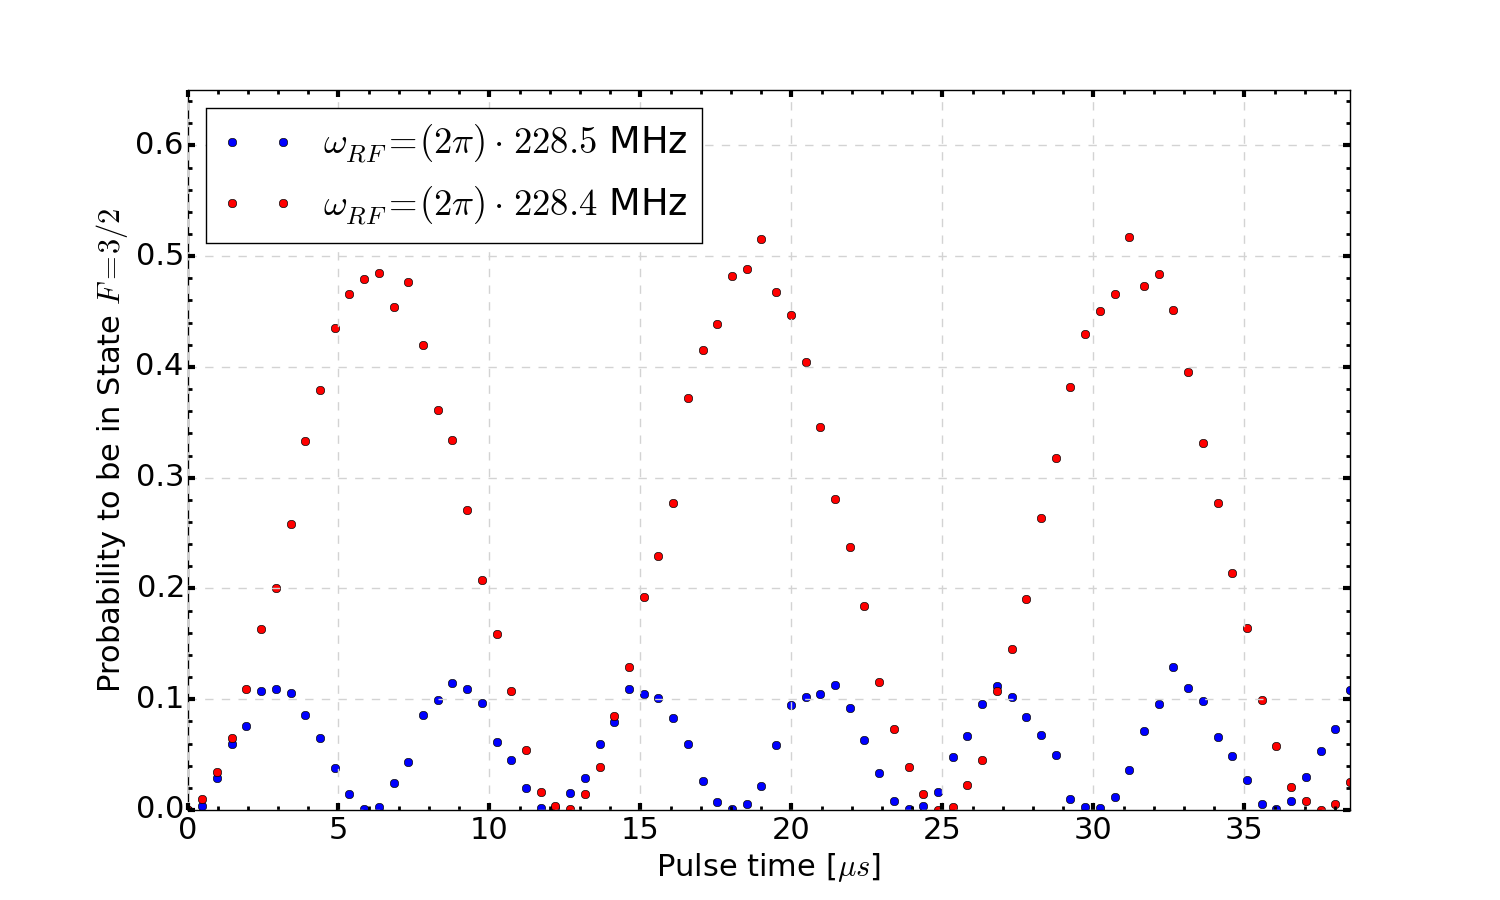
\includegraphics[angle=0, width=0.75\textwidth]
{./part1/interaction/RabiOscillations2_v3.png}
\else
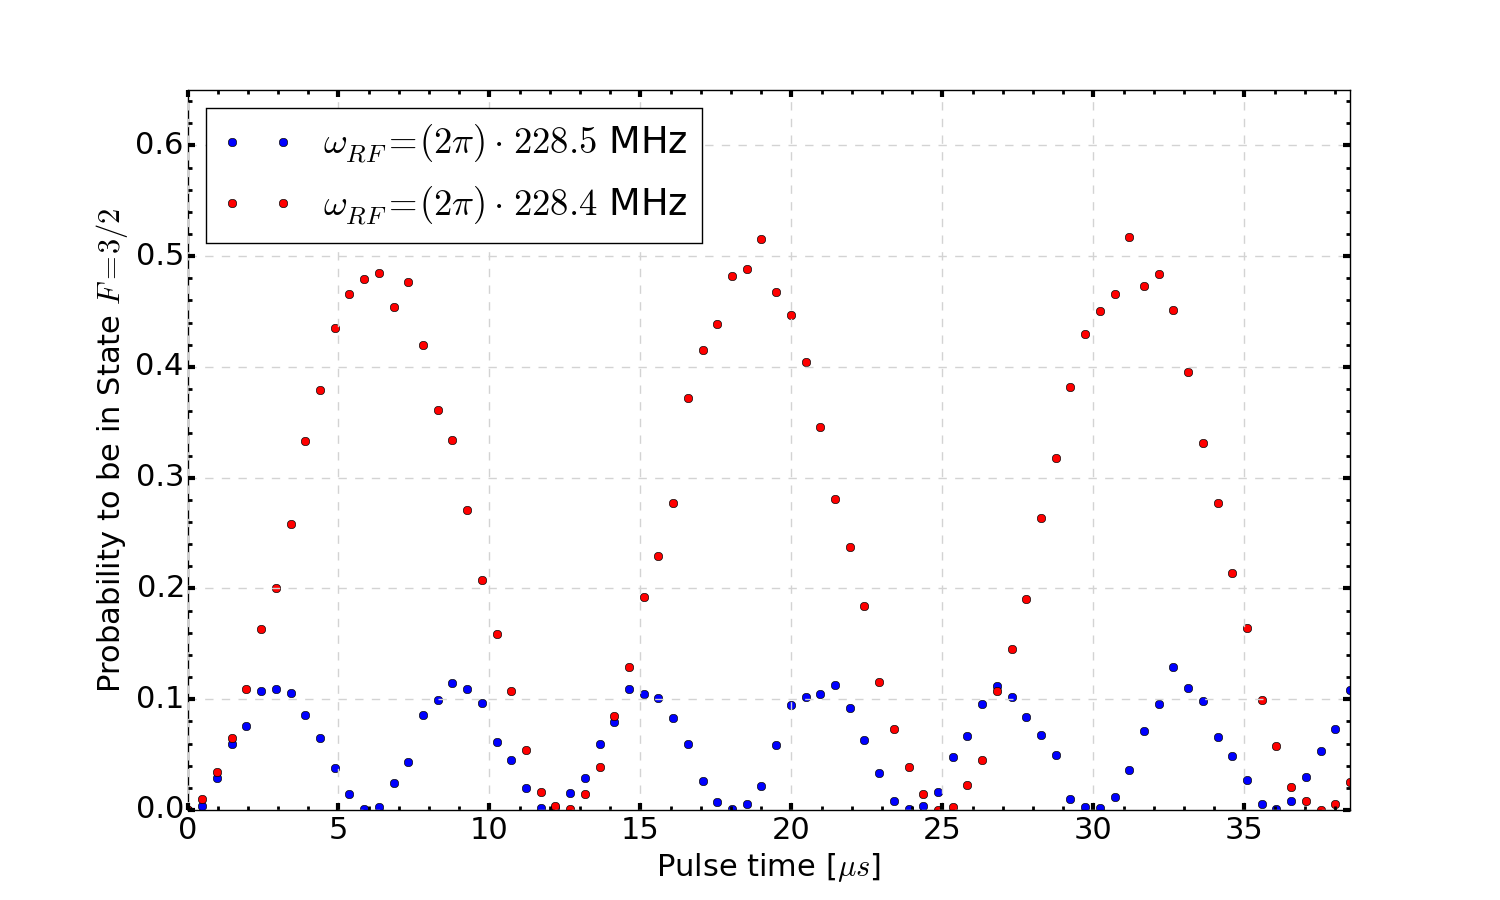
\includegraphics[angle=0, width=0.75\textwidth]
{./part1/interaction/RabiOscillations2_v3.eps}
\fi

\caption{You want to measure the transition frequency $f_0 = \frac{\omega_o}{2 \pi}$ between two states of a lithium atom by assessing Rabi oscillations. You prepare a cold cloud of lithium atoms in the state $\ket{1}$ (the so-called $\ket{F=1/2}$ state) and you can apply an electromagnetic pulse of fixed intensity and variable duration $\tau$. Finally, you measure the number of atoms in the state $\ket{2}$ (the so-called $\ket{F=3/2}$ state). You know that the frequency difference between these two levels is close to $2 \pi \cdot 228.5 \mbox{MHz}$, therefore you apply an electromagnetic pulse with a frequency close to this value: initially with a frequency $\omega_1 = 2 \pi \cdot 228.5 \mbox{MHz}$, then you repeat the measurements with frequency $\omega_2 = 2 \pi \cdot 228.4 \mbox{MHz}$. The result is shown in the presented figure. What is the transition frequency $f_0 = \frac{\omega_o}{2 \pi}$ between the two states of the lithium atom?}
\label{figPart1InteractionQuestionFreq}
\end{figure}